\documentclass{VUMIFPSkursinis}
\usepackage{algorithmicx}
\usepackage{algorithm}
\usepackage{algpseudocode}
\usepackage{amsfonts}
\usepackage{amsmath}
\usepackage{bm}
\usepackage{caption}
\usepackage{color}
\usepackage{float}
\usepackage{graphicx}
\usepackage{listings}
\usepackage{subfig}
\usepackage{wrapfig}
\usepackage{sectsty}

\usepackage{enumitem}
%PAKEISTA, tarpai tarp sąrašo elementų
\setitemize{noitemsep,topsep=0pt,parsep=0pt,partopsep=0pt}
\setenumerate{noitemsep,topsep=0pt,parsep=0pt,partopsep=0pt}
\allsectionsfont{\centering}
% Titulinio aprašas
\university{Vilniaus universitetas}
\faculty{Matematikos ir informatikos fakultetas}
\department{Programų sistemų katedra}
\papertype{Programų sistemų inžinerijos I laboratorinis darbas}
\title{Socialinis Vilniaus universiteto tinklalapis}
\titleineng{SocialVU}
\status{2 kurso 4 grupės studentai}
\author{Andrejus Voitovas}
\secondauthor{Eglė Puodžiūnaitė}
\thirdauthor{Kasparas Kralikas}
\fourthauthor{Ieva Vizgirdaitė} % Pridėti antrą autorių
\supervisor{asist. dr. Vytautas Valaitis}
\date{Vilnius – \the\year}

% Nustatymai
% \setmainfont{Palemonas}   % Pakeisti teksto šriftą į Palemonas (turi būti įdiegtas sistemoje)
\bibliography{bibliografija}

\begin{document}
% PAKEISTA
\maketitle
\cleardoublepage\pagenumbering{arabic}
\setcounter{page}{2}
\sectionnonum{ANOTACIJA}
Šiame dokumente pateikiami funkciniai ir nefunkciniai reikalavimai sistemai. Sistema ana-
lizuojama taikant ICONIX metodą. Apibrėžiamas struktūrinis dalykinės srities modelis, paaiški-
namos sistemoje naudojamos sąvokos. Taip pat aprašomos sistemoje atliekamos užduotys, anali-
zuojami pagrindiniai ir alternatyvūs užduoties scenarijai, naudojant sekų diagramas. Apibrėžiama
techninė kuriamos sistemos architektūra bei testavimo planas ir scenarijai.
\newpage
%TURINYS
\tableofcontents

\sectionnonum{ĮVADAS}
\textbf{Tikslas}  - sukurti socialinio tinklalalapio prototipą, kurį įgyvendinus būtų palengvinta universiteto bendruomenės komunikaciją.\\
\textbf{Temos aktualumas} \\
Šiuo metu studentams dėstytojų skelbiama informacija yra išbarstyta internete, kurią surasti užima galybes laiko. Yra atskiras universiteto naujienų puslapis, kiekvienas dėstytojas turi savo asmeninį tinklalapį, atskiras elektroninis paštas. Tiek dėstytojui pasiekti studentus, tiek studentui dėstytoją yra komplikuota ir nepatogu.\\
\textbf{Dalykinė sritis}\\
Socialinis Vilniaus Universiteto tinklapis.\\
\textbf{Probleminė sritis}\\
Socialinis Vilniaus Universiteto tinklapis suteiktų galimybę greitai ir paprastai pasiekti šio universiteto dėstytojų puslapius, informaciją juose, susisiekti sus pačiais dėstytojais. Pagrindinis tinklalapio išskirtinumas - greitai ir patogiai pasiekiama informacija, viskas vienoje vietoje. Itin patogus valdymas dėstytojams.\\
 \textbf{Naudoti dokumentai}\\
 Dokumentas parengtas pagal kursinio darbo reikalavimus naudojant Latex programą ir jau sukurtus šablonus.\\
 \textbf{Darbo pagrindas} \\ 
Dokumentas parengtas kaip Programų sistemų inžinerijos I laboratorinis darbas.
\newpage
\sectionnonum{KURIAMOS SISTEMOS ARCHITEKTŪRA}
EGLĖ
\newpage
\section{LOGINIS PJŪVIS}
Loginį pjūvį sudaro klasių diagramos, kurios naudojamos pavaizduoti sistemos architektūros projektavimo etapus.
\subsection{Esybių klasių diagrama (nulinis lygis)}
\begin{figure}[H]
\centering
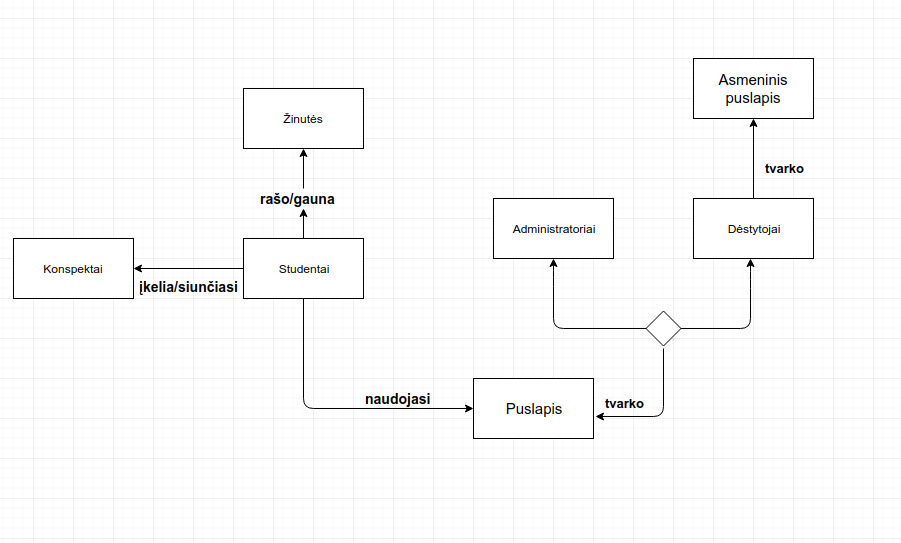
\includegraphics[width=\linewidth]{img/dalykine.png}
\label{fig:dalykine}
\caption{Dalykinė srities UML diagrama}
\end{figure}
Esybių diagramoje \ref{fig:dalykine} vaizduojamos esybių sąsajos. Pagrindinė esybė Naudotojas,
kuris gali būti Studentas, Dėstytojas arba Administratorius. Studentas turi galimybę naudotis pagrindinėmis puslapio funkcijos, o dėstytojai ir administratoriai pateikti naudingą studentams meždiagą. Taip pat studentai bei dėstytojai gali komunikuoti tarpusavyje nesinaudojant trečiųjų šalių komunikacinėmis priemonėmis. Administratoriai, savo ruožtu, pateikia informaciją apie renginius, naujienas ir D.U.K.
\subsection{Klasių diagrama (pirmas lygis)}
\begin{figure}[H]
\centering
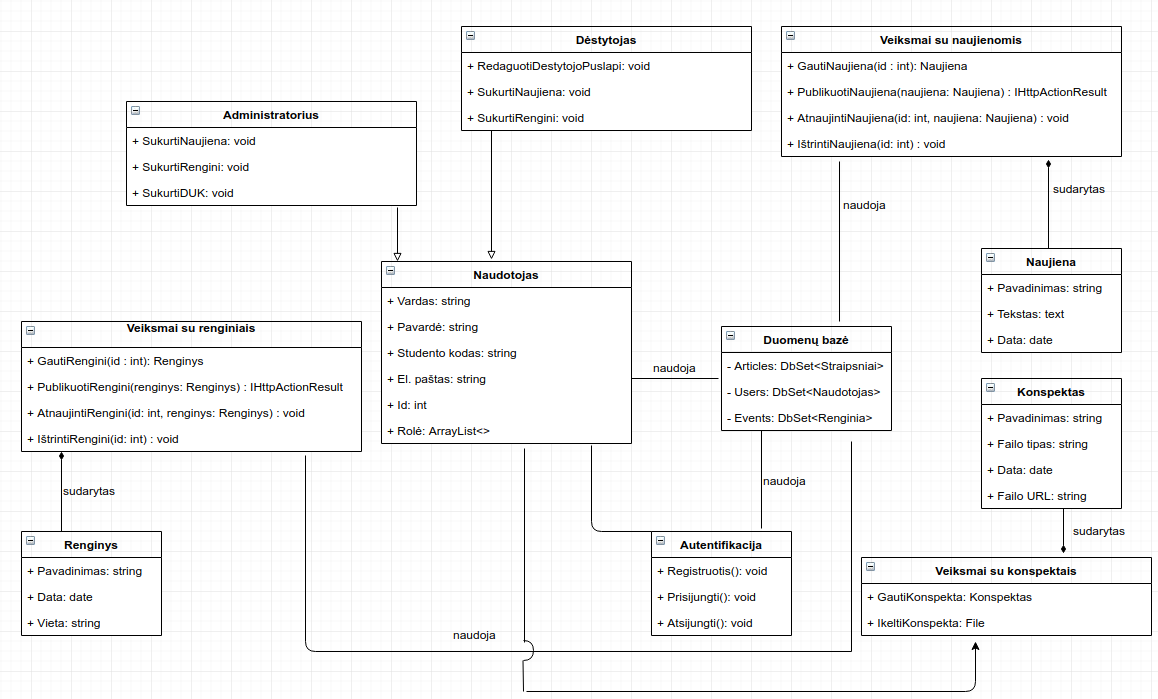
\includegraphics[width=\linewidth]{img/pagrindine.png}
\label{fig:pagrindine}
\caption{Dalykinė srities UML diagrama}
\end{figure}
Pagrindinį programos funkcionalumą užtikrina šios klasės: Studentas, Dėstytojas, Administratorius, Reitingas, Dėsytotojo puslapis, Naujienos, Autentifikacija, Duomenų bazė,
D.U.K., Renginiai. Veikimą įgyvendinačių klasių tarpusavio bendradarbiavimas vaizduojamas asociacija, ge-
neralizacija, kompozicija bei kardinalumus \ref{fig:pagrindine}.
\newpage
\section{UŽDUOČIŲ PJŪVIS}
IEVA
\newpage
\section{KŪRIMO PJŪVIS}
KASPARAS
\newpage
\section{FIZINIS PJŪVIS}
KASPARAS
\newpage
\section{PROCESO PJŪVIS}
Procesų pjūvis sudarytas iš sekų ir veiklos diagramų. Diagramose parodoma, kokie procesai
vyksta sistemoje bei išreiškiama komunikacija tarp jų.
\subsection{Proceso sekų diagramos}
Procesų sekų diagramose, atsispindi procesai, kurie yra vykdomi sistemoje. Iš proceso
sekų diagramos galima matyti, kokie komponentai dalyvauja vykdyme, kaip procesas vykdomas.
\subsubsection{Proceso „Prisijungimas” sekų diagrama}
\begin{figure}[H]
	\centering
	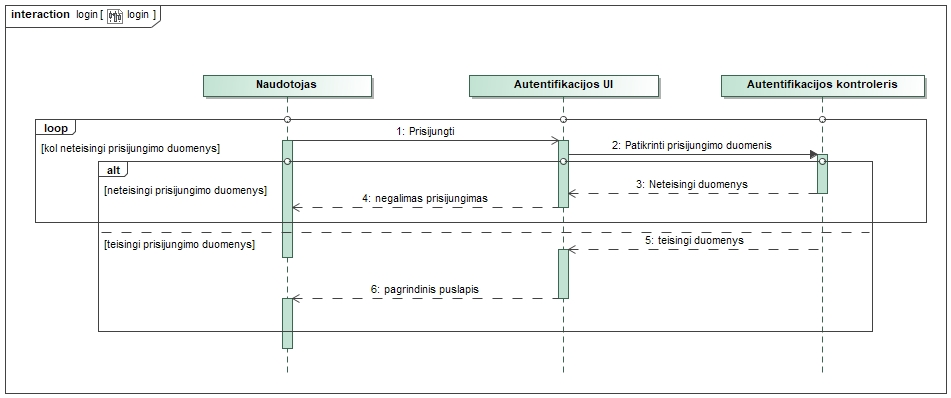
\includegraphics[width=\linewidth]{img/login.jpg}
	\caption{Proceso „Prisijungimas” sekų diagrama}
	\label{fig:login}
\end{figure}
Pagal \ref{fig:login} pav. diagramą matoma, kad procesas prasideda naudotojo paspaudimu ant nuorodos įgalinančios prisijungimą. Autentifikacijos
UI gautus duomenis siunčia patikrinimui į autentifikacijos kontrolerį. Iš kontrolerio
gaunamas atsakymas, ar duomenys teisingi ar ne. Jei duomenys klaidingi, vartotojui išmetamas pranešimas,
jog prisijungti negalima ir jis vėl gali kartoti prisijungimo procesą. Jei duomenys teisingi,
naudotojas yra nukreipiamas į pagrindinį puslapį.
\subsection{Veiklos diagramos}
Veiklos diagramos padeda suprasti dinaminį sistemos
veikimą, parodo, kokie veiksmai atliekami vykdant konkrečią veiklą, galimus vykdymo atvejus.
\subsubsection{Žinutės išsiuntimo veiklos diagrama}
\begin{figure}[H]
	\centering
	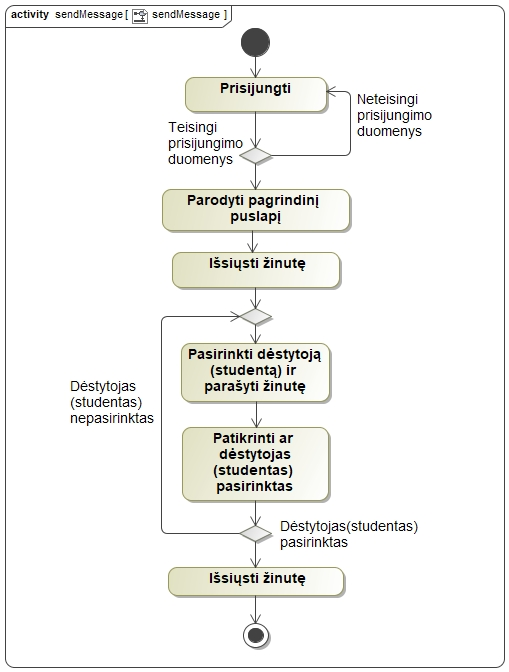
\includegraphics[scale=0.65]{img/sendMessage.jpg}
	\caption{Žinutės išsiuntimo veiklos diagrama}
	\label{fig:sendMessage}
\end{figure}
\ref{fig:sendMessage} pav. diagramoje matomas, žinutės išsiuntimo dėstytojui procesas. Procesas prasideda naudotojo
nuorodos paspaudimu, kreipiančios į žinutės išsiuntimo formą. Naudotojas pateikia parašo žinutę bei pasirenka dėstytoją, tuomet duomenys siunčiami patikrinimui. Jei dėstytojas nebuvo pasirinktas, naudotojas nukreipiamas
atgal į žinutės siuntimo formą. Jei duomenys atitinka visus reikalavimus, tada žinutė išsiunčiama.
\subsubsection{Naujienos paskelbimo veiklos diagrama}
\begin{figure}[H]
	\centering
	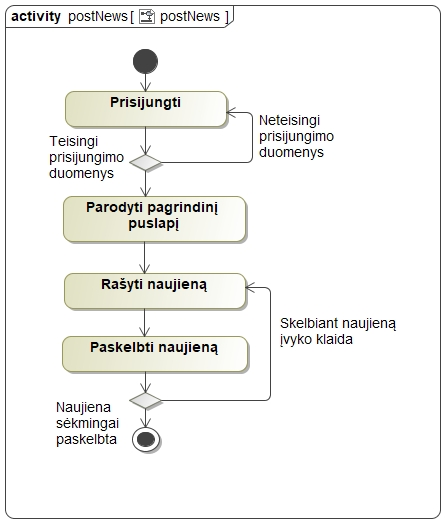
\includegraphics[scale=0.65]{img/postNews.jpg}
	\caption{Naujienos paskelbimo veiklos diagrama}
	\label{fig:postNews}
\end{figure}
\ref{fig:postNews} pav. diagramoje matomas, naujienos paskelbimo procesas. Procesas prasideda naudotojo prisijungimu. Neteisingai suvedus prisijungimo duomenis naudotojas vėl nukreipiamas į prisjungimą, kitu atveju jis nukreipiamas į pagridinį puslapį bei pasirenka naujienos paskelbimo nuorodą. Naudotojas parašo naujieną bei ją paskelbia. Jei skelbiant naujieną įvyksta klaida jis nukreipiamas į naujienos rašymo formą, kitu atveju naujiena paskelbiama.
\newpage
\section{RYŠIAI TARP PJŪVIŲ}
EGLĖ
\newpage
\sectionnonum{IŠVADOS}
KASNORS
\newpage
\sectionnonum{ŠALTINIAI}
KASNORS
\end{document}